% Chapter 2
\section[One dimension: correlation, direction, and causation]{One-Dimensional Linear Regression: Correlation, Direction, and Causation Inside a Single Line}\label{sec:onedim}

Start from the simplest model --- no intercept, a single feature:
\begin{equation}\label{eq:1d-model}
  y_i = b\, x_i + \varepsilon_i, \qquad i = 1, \dots, n,
\end{equation}
where $b \in \R$ is the parameter to estimate. This chapter does two things: first, \textit{from the regression viewpoint}, it shows how $b$ measures the correlation between $x$ and $y$; then, \textit{from the variance viewpoint}, it shows how the same straight line exposes the \textit{directionality} of correlation, and why it cannot tell you causation.

\subsection{Least squares: generalizing the mean into a line}\label{sec:1d-ls}

Forget statistics for a moment. Write the fitting problem as an optimization problem: find $b$ that minimizes the sum of squared residuals
\begin{equation}\label{eq:1d-rss}
  S(b) = \sum_{i=1}^n (y_i - b\, x_i)^2 .
\end{equation}
Differentiate with respect to $b$ and set to zero:
\[
  \frac{dS}{db} = -2 \sum_{i=1}^n x_i (y_i - b x_i) = 0
  \quad\Longrightarrow\quad
  \boxed{\;\hat{b} = \frac{\sum_{i=1}^n x_i y_i}{\sum_{i=1}^n x_i^2}\;}
\]
The second derivative $\frac{d^2 S}{db^2} = 2 \sum_i x_i^2 > 0$ (as long as $x$ is not identically zero), so this is the unique global minimizer. No initial guess, no learning rate, no local minima --- convexity settles everything at once.

Look at two extremes to build intuition. If $x_i \equiv 1$, then $\hat{b} = \bar{y}$: \textbf{least squares is the generalization of the mean} --- the sample mean is precisely the constant that minimizes the sum of squared deviations. If the model has an intercept, $y_i = a + b x_i + \varepsilon_i$, exactly the same differentiation gives
\begin{equation}\label{eq:1d-slope}
  \hat{b} = \frac{\Cov_n(x, y)}{\Var_n(x)}, \qquad \hat{a} = \bar{y} - \hat{b}\,\bar{x},
\end{equation}
i.e., the regression line must pass through the data centroid $(\bar{x}, \bar{y})$. Read \eqref{eq:1d-slope} slowly: \textit{the slope is the degree to which $x$ and $y$ vary together, divided by the degree to which $x$ varies on its own}. The most quoted formula in all of applied statistics is nothing more than one differentiation. Note that no error distribution has been assumed so far --- least squares, up to this point, is purely geometric optimization.

\subsection{The regression viewpoint: the slope \emph{is} the correlation coefficient}\label{sec:1d-corr}

Now standardize the data. Write $\sigma_x = \sqrt{\Var_n(x)}$, $\sigma_y = \sqrt{\Var_n(y)}$; the Pearson (1896) correlation coefficient\cite{pearson1896} is
\begin{equation}\label{eq:rho}
  r = \frac{\Cov_n(x, y)}{\sigma_x \, \sigma_y} \in [-1, 1].
\end{equation}
(By Cauchy--Schwarz, $|\Cov_n(x,y)| \le \sigma_x \sigma_y$, so $r$ indeed lies in $[-1,1]$.) Substituting into \eqref{eq:1d-slope}:
\begin{equation}\label{eq:slope-rho}
  \boxed{\;\hat{b} = r \, \frac{\sigma_y}{\sigma_x}\;}
\end{equation}

This single line is the hub of the chapter; it says three things:

\begin{enumerate}[label=(\arabic*)]
  \item \textbf{The \textit{strength} of correlation} ($|r|$, dimensionless, symmetric, unit-free) determines the \textit{steepness} of the regression line in standard-deviation units: $\frac{\hat{b}\, \sigma_x}{\sigma_y} = r$. Moving $x$ by one standard deviation moves the prediction $\hat{y}$ by $r$ standard deviations.
  \item \textbf{The symmetry of $r$ vs.\ the directionality of regression}: $r$ is unchanged under swapping $x$ and $y$; but the regression line $y \sim x$ (predicting $y$ from $x$) and the regression line $x \sim y$ are two \textit{different} lines (see Section~\ref{sec:1d-direction}).
  \item \textbf{Goodness of fit}: the coefficient of determination
  \begin{equation}\label{eq:r2-rho2}
    R^2 = 1 - \frac{\sum_i e_i^2}{\sum_i (y_i - \bar{y})^2} = r^2,
  \end{equation}
  i.e., the proportion of the sample variance of $y$ explained linearly by $x$ is exactly the square of the correlation coefficient (an identity that presumes the intercept is fitted --- without one it fails). $R^2$ measures correlation, while $r$ also carries a sign (direction).
\end{enumerate}

\begin{example}[Galton's height regression]\label{ex:galton}
Galton (1886) studied the heights of 205 parent couples and 928 adult children, predicting child height $y$ from mid-parent height $x$, and obtained a regression equation of approximately $y = 0.516\,x + 33.73$ (inches)\cite{galton1886}. The two generations have nearly identical standard deviations (about 3.3 inches), so in standard-deviation units the slope is simply $r \approx 0.5$: parents one standard deviation taller than average have children who are on average only half a standard deviation taller. Children of tall parents \textbf{regress toward mediocrity}, and so do children of short parents --- hence the name ``regression toward the mean.'' This is not a law of biology; it is the arithmetic of \eqref{eq:slope-rho}: as long as $|r| < 1$ and each variable's dispersion stays put, extremes necessarily fall back.\end{example}

\begin{remark}
``Regression to the mean'' is the ancestor of all statistical fallacies: the Sports Illustrated jinx, second-exam slump, and triumph-of-mediocrity arguments \`a la Secrist (1933) are all, at bottom, noise mistaken for signal. Galton himself avoided the trap with subtler reasoning\cite{galton1886,stigler1986}.
\end{remark}

\begin{figure}[htbp]
  \centering
  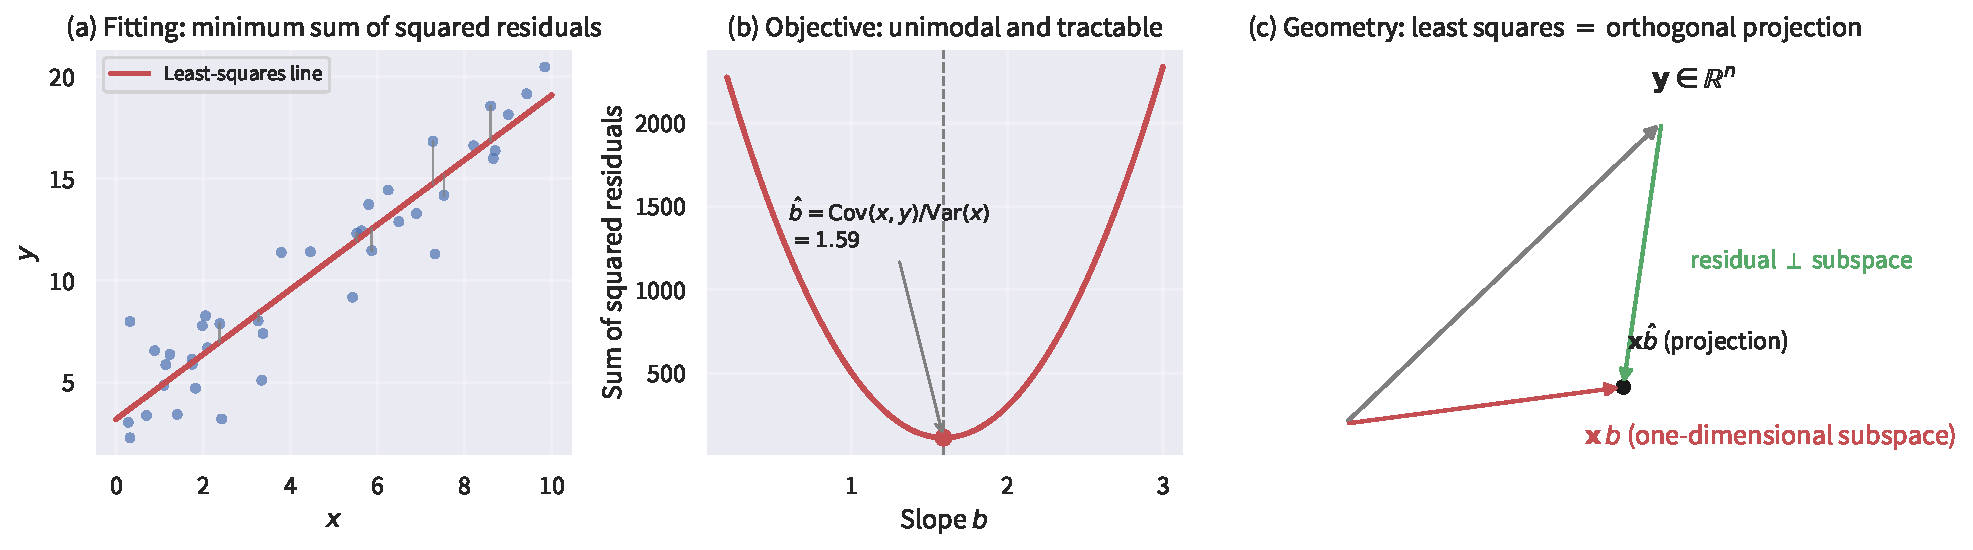
\includegraphics[width=\linewidth]{figures/ch2_leastsq.pdf}
  \caption{Three faces of one-dimensional least squares: (a) fitting --- the squared sum of the residuals (vertical bars) is minimized; (b) optimization --- the objective is unimodal in the slope $b$, and $\hat b=\Cov(x,y)/\Var(x)$ solves it in one step; (c) geometry --- $\x\hat b$ is the orthogonal projection of $\y$ onto a one-dimensional subspace, with residuals $\perp$ to the subspace.}
  \label{fig:ch2-leastsq}
\end{figure}

\subsection{The variance viewpoint: where correlation comes from, and what it means}\label{sec:1d-var}

Look again through a different lens. Treat $y$ in \eqref{eq:1d-model} as a random variable $y = bx + \varepsilon$, and assume $\Cov(x, \varepsilon) = 0$ (i.e., $x$ carries no component of $y$'s noise --- this \textit{is itself a directional assumption}!). The algebra of variance gives
\begin{equation}\label{eq:var-decomp}
  \Var(y) = b^2 \Var(x) + \Var(\varepsilon).
\end{equation}
\textbf{The fluctuation of $y$ splits into two parts: the part carried by $x$, $b^2\Var(x)$, and the irreducible noise $\Var(\varepsilon)$.} Immediately,
\begin{equation}\label{eq:r2-var}
  R^2 = \frac{b^2 \Var(x)}{\Var(y)} = 1 - \frac{\Var(\varepsilon)}{\Var(y)},
\end{equation}
which converges with \eqref{eq:r2-rho2} from a different route: $r^2$ is simultaneously ``goodness of fit at the sample level'' and ``the population share of explained variance.'' This is the first payoff of the variance viewpoint --- \textit{correlation is, in essence, a transfer of variance}.

The second payoff is deeper. In \eqref{eq:var-decomp}, the sign of $b$ describes ``how fluctuations of $x$ get translated into fluctuations of $y$.'' But if the true structure is $y$ causing $x$, and you regress $y \sim x$ anyway, you still obtain the same $\hat{b} \approx r\,\sigma_y/\sigma_x$. Correlation is \textit{completely blind} to the direction of generation --- the theme of the next section.

\subsection{Directionality: two regression lines, and one major axis}\label{sec:1d-direction}

Standardize both $x$ and $y$ (mean zero, variance one); then the \textbf{regression coefficients} in both directions equal $r$:
\[
  \text{coefficient of } y \sim x = r,
  \qquad
  \text{coefficient of } x \sim y = r,
  \qquad
  \text{product of the two} = r^2 < 1 \; (|r| < 1).
\]
(The second equality concerns the ``coefficient,'' not the ``slope'': the regression of $x$ on $y$ solves to $x = r\,y$, which read with $y$ as the independent variable indeed has coefficient $r$.) In other words, unless $|r| = 1$ (perfect linearity, no noise), \textbf{``the line that predicts $y$ from $x$'' and ``the line that predicts $x$ from $y$'' are two different straight lines}. One terminological point must be made precise: \textit{regression coefficients} and \textit{geometric slopes drawn in the same coordinate system} are not the same thing. On the original scale, the two regression coefficients are respectively
\[
  b = r\,\frac{\sigma_y}{\sigma_x} \;(y \sim x), \qquad
  b' = r\,\frac{\sigma_x}{\sigma_y} \;(x \sim y),
  \qquad b\, b' = r^2 < 1,
\]
--- the product of the coefficients is $r^2$, which is Galton's ``regression toward the mean'' arithmetic; but if both lines are drawn in the same ``$x$ horizontal, $y$ vertical'' coordinate system, the second must be rewritten as $y = \dfrac{\sigma_y}{r\,\sigma_x}\,x$, so the \textbf{geometric slopes} are $r\,\sigma_y/\sigma_x$ and $\sigma_y/(r\,\sigma_x)$, whose product is $(\sigma_y/\sigma_x)^2$ --- identically $1$ only when $\sigma_x = \sigma_y$ (including the standardized case). Both products are correct; they simply measure two different questions: the former asks ``how much does each direction's prediction shrink,'' the latter asks ``the opening angle between the two lines on the plot.'' A bivariate-normal-ish point cloud approximates an ellipse, and the two regression lines are respectively: the line minimizing vertical residuals and the line minimizing horizontal residuals --- neither coincides with the ellipse's major axis (the major axis corresponds to PCA, which minimizes \textit{perpendicular} distance). Burn Figure~\ref{fig:ellipse} into your mind, and ``regression has direction, correlation does not'' ceases to be a slogan.

\begin{figure}[htbp]
\centering
\resizebox{0.72\linewidth}{!}{%
\begin{tikzpicture}[>=Stealth, scale=2.6]
  % point-cloud ellipse
  \draw[thick, color=black!60, rotate around={35:(0,0)}] (0,0) ellipse (2.2 and 1.0);
  \fill[black!40] (35:1.3) circle (0.02);
  \fill[black!40] (215:0.9) circle (0.02);
  \fill[black!40] (35:-0.8) circle (0.02);
  \fill[black!40] (215:1.6) circle (0.02);
  \fill[black!40] (35:0.3) circle (0.02);
  \fill[black!40] (215:-1.4) circle (0.02);
  \draw[->] (-2.9,0) -- (2.9,0) node[below left] {$x$};
  \draw[->] (0,-2.3) -- (0,2.3) node[below left] {$y$};
  % major axis
  \draw[thick, dashed, color=black!50] (-2.35,-1.65) -- (2.35,1.65) node[above right=-2pt] {major axis (PCA)};
  % regression line y~x: slope tan(35°) * (short/long) ≈ 0.7*0.455 ≈ 0.32 → approximated with rotate
  \draw[very thick, color=accent] (-2.7,-0.86) -- (2.7,0.86) node[below right=-2pt] {regression $y \sim x$};
  % regression line x~y
  \draw[very thick, color=red!70!black] (-1.35,-2.2) -- (1.35,2.2) node[above=-2pt] {regression $x \sim y$};
\end{tikzpicture}}
\caption{A standardized bivariate-normal point cloud (ellipse). Neither regression line coincides with the major axis: $y \sim x$ minimizes vertical residuals, $x \sim y$ minimizes horizontal residuals, and the major axis minimizes perpendicular residuals. Regression is a \textit{directed} operation; the correlation coefficient $r$ is not.}
\label{fig:ellipse}
\end{figure}

Directionality also has a purely algebraic statement: the decompositions $\Var(y) = b^2\Var(x) + \Var(\varepsilon)$ from \eqref{eq:var-decomp} and $\Var(x) = \tilde{b}^2 \Var(y) + \Var(\tilde\varepsilon)$ (regressing $x$ on $y$) can hold simultaneously, and each has $R^2 = r^2$. The two directions carry the same ``explanatory power'' --- the variance expression of correlation's symmetry; the slopes differ --- the expression of directionality.

\subsection{Causation: what a correlation coefficient can never give you}\label{sec:1d-causality}

Why can't $r$ assert causation? Because at least three fundamentally different generative mechanisms produce \textit{exactly the same} correlation coefficient:

\begin{center}
\begin{tabular}{@{}lll@{}}
\toprule
Structure & Generative process & Observed correlation \\
\midrule
$x$ causes $y$ & $y = bx + \varepsilon$ & $r \neq 0$ \\
$y$ causes $x$ & $x = \tilde{b} y + \tilde\varepsilon$ & $r \neq 0$ (the same $r$) \\
Common cause $z$ & $x = c z + u,\;\; y = d z + v$ & $r = \mathrm{sign}(cd)\cdot(\text{determined by } c,d)$ \\
\bottomrule
\end{tabular}
\end{center}

The data themselves have zero power to distinguish these three cases --- a corollary of Reichenbach's (1956) \textbf{common-cause principle}: if $A$ and $B$ are statistically correlated, then either $A$ causes $B$, or $B$ caused $A$, or there is a common cause $C$\cite{reichenbach1956}. The principle provides the enumeration but not the decision --- the decision must come from knowledge beyond the data.

Wright (1921) was the first to turn this into a calculus\cite{wright1921}. His \textbf{path analysis} says: on a given causal graph (whose arrows must be drawn beforehand from experiment, temporal order, or domain knowledge), the correlation between any two variables equals the sum, over all legal paths connecting them, of the products of the path coefficients. Hence:
\begin{itemize}
  \item \textit{Forward use}: given a causal hypothesis, use the observed correlations to \textit{test} it (fit; residual correlations should vanish);
  \item \textit{Reverse use}: inferring causal structure from correlations alone is beyond statistics --- ``the validity of these conclusions depends upon knowledge external to the method'' (the substance of Wright's original remark\cite{wright1921}).
\end{itemize}

More than a century later, this criterion remains the root of all causal inference (structural equation models, DAGs, do-calculus, difference-in-differences, instrumental variables): \textbf{regression outputs conditional association; reading a coefficient as a causal effect requires an identification strategy} --- randomization, natural experiments, or the untestable ``no unmeasured confounding'' assumption. This boundary lies beyond the range of any $t$-statistic.

\begin{keybox}[Takeaways of this chapter]
\begin{itemize}
  \item The one-dimensional least-squares slope $\hat{b} = \Cov_n(x,y)/\Var_n(x) = r\,\sigma_y/\sigma_x$: regression generalizes the mean, the correlation coefficient is its standardized form, and $R^2 = r^2$ is both goodness of fit and the share of explained variance.
  \item Variance viewpoint: $\Var(y) = b^2\Var(x) + \Var(\varepsilon)$ --- correlation is the transfer of variance; $\Cov(x,\varepsilon)=0$ is already a directional assumption.
  \item Directionality: $y \sim x$ and $x \sim y$ are two different regression lines (the product of regression coefficients is $r^2$; the product of geometric slopes drawn in one coordinate system is $(\sigma_y/\sigma_x)^2$, equal to $1$ only when $\sigma_x = \sigma_y$); correlation is symmetric, regression is not.
  \item Causation: at least three structures produce the same $r$; the common-cause principle enumerates them, path analysis provides ``a calculus given external causal knowledge,'' but the data alone can never decide the direction.
\end{itemize}
\end{keybox}
